% This file was created by tikzplotlib v0.8.5.
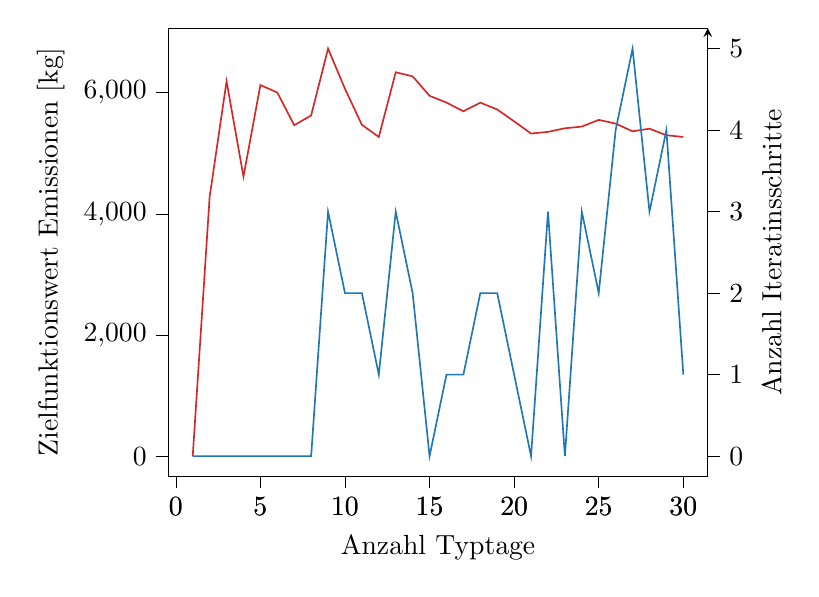
\begin{tikzpicture}

\definecolor{color0}{rgb}{0.83921568627451,0.152941176470588,0.156862745098039}
\definecolor{color1}{rgb}{0.12156862745098,0.466666666666667,0.705882352941177}

\begin{axis}[
tick align=outside,
tick pos=left,
x grid style={white!69.01960784313725!black},
xlabel={Anzahl Typtage},
xmin=-0.45, xmax=31.45,
xtick style={color=black},
y grid style={white!69.01960784313725!black},
ylabel={Zielfunktionswert Emissionen [kg]},
ymin=-336.316, ymax=7062.636,
ytick style={color=black}
]
\addplot [semithick, color0]
table {%
1 0
2 4279.83
3 6186.55
4 4614.23
5 6125.08
6 6001.56
7 5462.06
8 5623.22
9 6726.32
10 6062.47
11 5468.86
12 5268.05
13 6335.88
14 6268.44
15 5947.73
16 5835.1
17 5692.08
18 5834.42
19 5721.57
20 5525.86
21 5324.48
22 5352.07
23 5411.23
24 5439.31
25 5549.91
26 5489.18
27 5361.35
28 5404.43
29 5296.77
30 5268.05
};
\end{axis}

\begin{axis}[
axis y line=right,
tick align=outside,
x grid style={white!69.01960784313725!black},
xmin=-0.45, xmax=31.45,
xtick pos=left,
xtick style={color=black},
y grid style={white!69.01960784313725!black},
ylabel={Anzahl Iteratinsschritte},
ymin=-0.25, ymax=5.25,
ytick pos=right,
ytick style={color=black}
]
\addplot [semithick, color1]
table {%
1 0
2 0
3 0
4 0
5 0
6 0
7 0
8 0
9 3
10 2
11 2
12 1
13 3
14 2
15 0
16 1
17 1
18 2
19 2
20 1
21 0
22 3
23 0
24 3
25 2
26 4
27 5
28 3
29 4
30 1
};
\end{axis}

\end{tikzpicture}
